\subsection{Lietotāja grafiskās saskarnes apraksts}
Programmas logs ir apskatāms \ref{fig:vessel-extractor} attēlā. Programma sastāv no vairākiem laukiem.  Datu vizualizācijas lauks ir paredzēts datortomogrāfijas slāņu vizualizācijai, kā arī asinsvadu tīklojuma 3D modeļa vizualizācijai. To, kas tiek attēlots var pārslēgt ar pogām: 2D View (Datortomogrāfija slāņu skats), 3D View (asinsvadu tīklojuma 3D modeļa skats). 3D modeļa skatā modelis ir aplūkojums tikai tad kad ir segmentēti asinsvadi, kā arī ģenerēts 3D modelis.
\begin{figure}[h]
\begin{center}
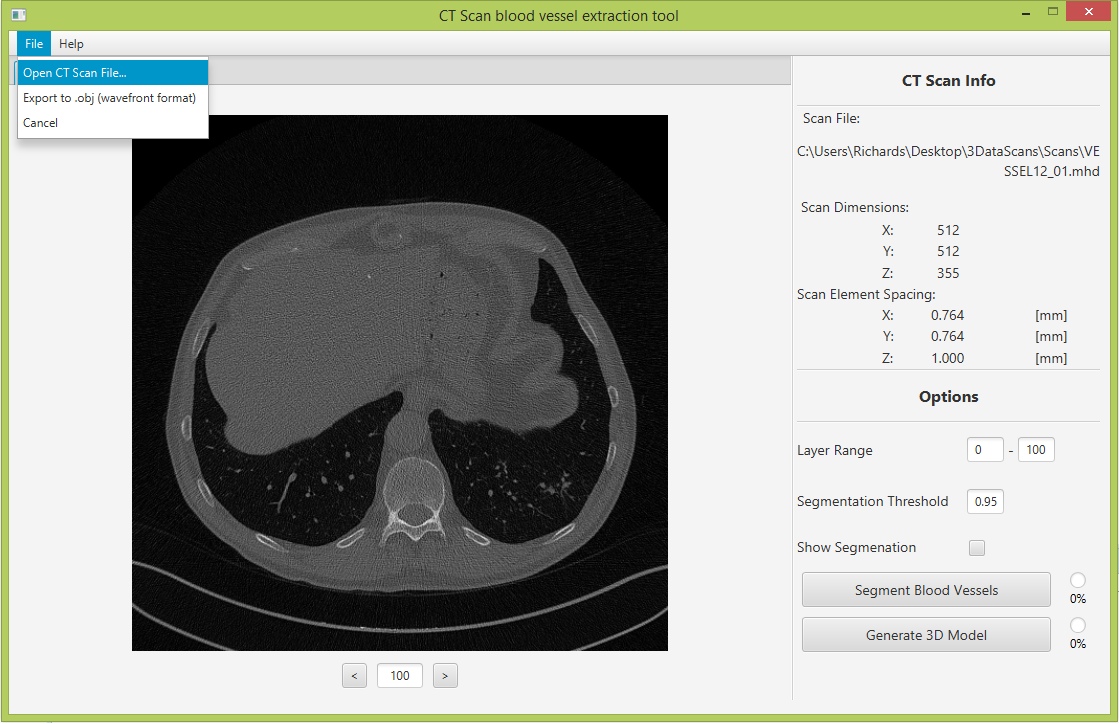
\includegraphics[scale=0.45]{img/vessel-extractor.png}
\caption{Asinsvadu segmentēšanas programmas logs}
\label{fig:vessel-extractor}
\end{center}
\end{figure}

Tomogrāfijas uzņēmumi tiek ielādēti izmantojot izvēlni: \textbf{File} $\rightarrow{}$  \textbf{Open CT Scan File...}. Izvēloties šo izvēlni tiek atvērts failu pārlūks (redzams \ref{fig:scan-select} attēlā), kas dažādām operētājsistēmām vizuāli atšķiras taču ir standartizēts operētājsistēmas ietvaros. Šajā logā var pārlūkot failu sistēmas mapes un pārvietoties pa tām, kā arī no attiecīgās mapes izvēlēties interesējošo datortomogrāfijas uzņēmumu. Kad datortomogrāfijas uzņēmums izvēlēts tas parādās datortomogrāfijas slāņa skata laukā, kā redzams \ref{fig:vessel-extractor} attēlā. Pārslēgšanās starp slāņiem veicama ar pogām zem šī laukā, kā arī ir iespējams tieši ievadīt slāņa kārtas skaitli (ja ievadītais skaitlis pārsniedz esošo slāņu daudzumu, tiek attēlots slānis ar pēdējo lielāko indeksu).

\begin{figure}[h]
\begin{center}
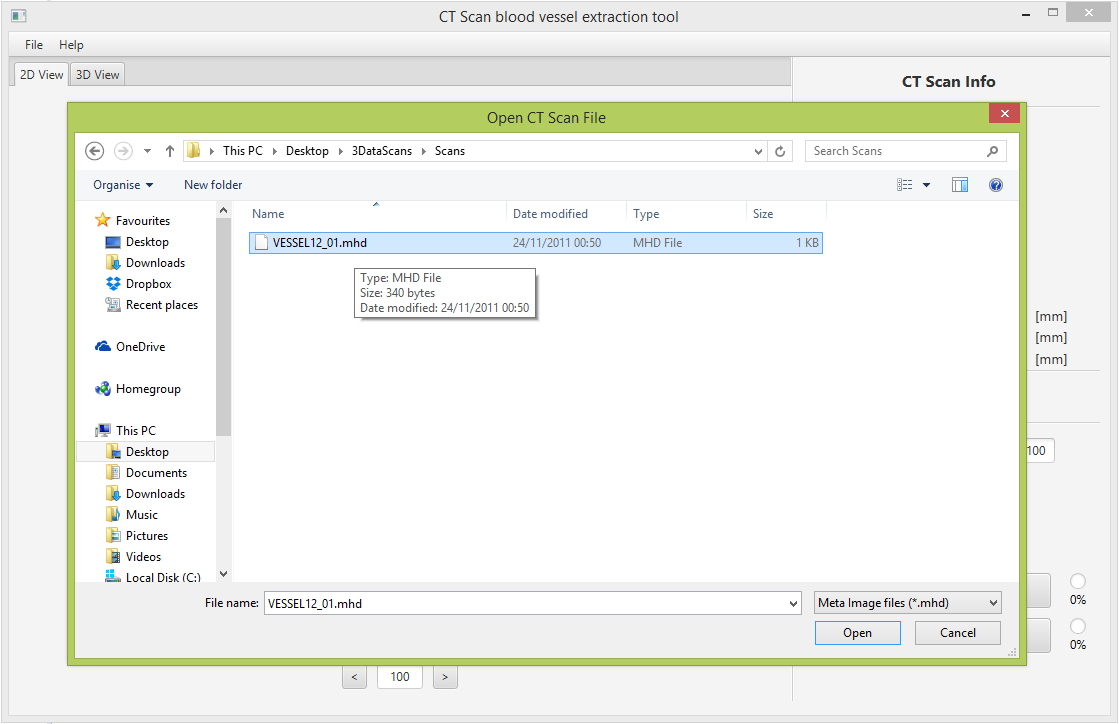
\includegraphics[scale=0.45]{img/scan-select.png}
\caption{Programmas datortomogrāfijas uzņēmuma failu izvēlnes logs}
\label{fig:scan-select}
\end{center}
\end{figure}

Labajā pusē atrodas \textbf{CT Scan info} lauks. Tajā tiek atspoguļota informācija par tomogrāfijas uzņēmumu: faila ceļš failu sistēmā, uzņēmuma izšķirtspēja visām dimensijām, kā arī fiziskais attālums starp pikseļiem milimetros. Zem šī lauka atrodas \textbf{Options} lauks, kurā atrodas uzstādījumi un vadības pogas:
\begin{itemize}
\item \emph{Layer Range} - Slāņu diapazons, kuram tiek veikta asinsvadu segmentēšana;
\item \emph{Segmentation Threshold} - Nosaka segmentēšanas jutību. Jo lielāka vērtība, jo mazāka jutība, taču nodrošina mazāku iespēju ka pikseļi tiek maldīgi uzskatīti par asinsvadiem. Sliekšņa vērtība ietekmē tikai 3D modeļa ģenerēšanu, tādēļ, lai pamainītu šo vērtību, atkārtota asinsvadu segmentēšana nav jāveic.
\item \emph{Show Segmentation} - Ļauj vizuāli iezīmēt segmentēšanas rezultātu tomogrāfijas uzņēmuma pie uzstādītās sliekšņa vērtības;
\item \emph{Segment Blood Vessels} - Poga, kas uzsāk asinsvadu segmentēšanas procesu. Šo procesu ietekmē tikai \emph{Layer Range} uzstādījums. Pa labi no pogas tiek attēlots segmentēšanas tekošais progress procentos.

\item \emph{Generate 3D model} - Poga, kas uzsāk asinsvadu 3D modeļa ģenerēšanas procesu. Šis process ir atkarīgs no asinsvadu segmentēšanas rezultāta, līdz ar to pirms 3D modeļa ģenerēšanas ir jābūt veiktai asinsvadu segmentēšanai. Process ir atkarīgs arī no uzstādītās segmentēšanas sliekšņa vērtības. Pa labi no pogas tiek attēlots segmentēšanas tekošais progress procentos.
\end{itemize}

Asinsvadu 3D modeļa ģenerēšanas rezultātu var aplūkot 3D skata laukā, kuru var atvērt ar pogu \emph{3D View}. 3D Skata lauks redzams \ref{fig:3D-view} attēlā. 3D modeli ir iespējams rotēt nospiežot ar kreiso peles taustiņu un velkot peli. 3D modeli ir iespējams pietuvināt un attālināt izmantojot peles rulli.
\begin{figure}[h]
\begin{center}
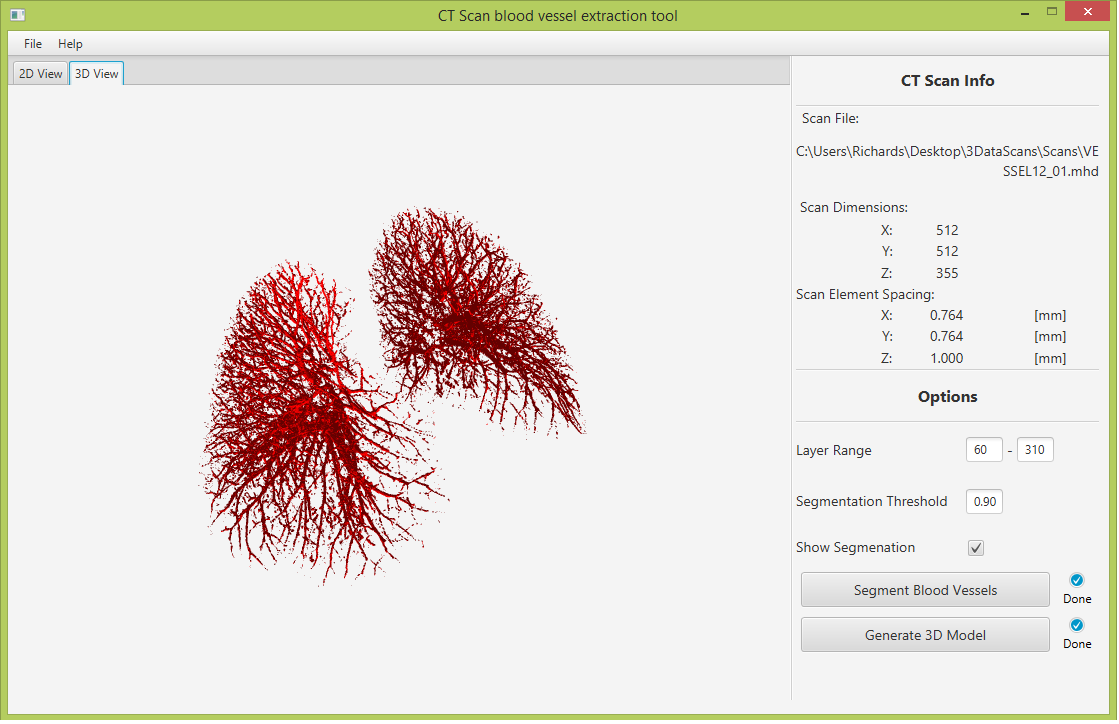
\includegraphics[scale=0.45]{img/vessels-3D.png}
\caption{Asinsvadu tīklojuma 3D modeļa skats}
\label{fig:3D-view}
\end{center}
\end{figure}

3D modeli ir iespējams eksportēt uz Wavefront failu formātu. Tas veicams ar izvēlnēm \textbf{File} $\rightarrow$ \textbf{Export to .obj (wavefront format)}. Eksportējot tiek atvērts failu pārlūka logs, kas ļauj norādīt mapi kurā saglabāt 3D modeli. Ģenerētā faila nosaukumam ir sekojoša struktūra: \emph{blood-vessel-model-9420151053.obj}. Ciparu virkne nosaukumā ir laika zīmogs. Cipari atbilst šādai secībai: datums, mēnesis, gads stunda, minūte.


